\chapter{Introduction}


\chaptermark{intro}
In this thesis we explore several new results relating to the existence of special metrics on certain compact K\"ahler manifolds admitting an effective algebraic torus action action. Our goal is to provide new examples to work with in the field, and further the understanding of canonical metrics on these types of manifolds. A K\"ahler manifold is a smooth manifold \(X\) adorned with mutually compatible Riemannian, complex, and symplectic structures. In this situation we call the Riemannian metric \(g\) the \textit{K\"ahler metric} on \(X\), and the symplectic form \(\omega\) the \textit{K\"ahler form}. An orbifold may be thought of as a generalization of a manifold, where we allow for very mild singularities, and the K\"ahler condition generalizes easily.

There are many reasons to study K\"ahler geometry. From the standpoint of algebraic geometry, every smooth complex projective variety inherits a K\"ahler structure. From a differential geometric perspective, K\"ahler manifolds are a particularly well-behaved class of Riemannian manifolds, and are a rich enough class to contain many interesting examples. There are also motivations from theoretical physics: the various models of our universe in string theory ask for extra planck-scale dimensions, and certain K\"ahler manifolds are the best fit for the shape of these dimensions.

Historically it has been an important problem in K\"ahler geometry to investigate which K\"ahler manifolds admit nice K\"ahler metrics. Generally what we mean here by ``nice" depends on context. For naive motivation consider the real 2-sphere see Figure 1. Most would have in their mind the standard embedding \(S^2 = \{ x^2+y^2+z^2 = 1 \} \subset \RR^3\). There are however many choices of smooth embedding, each one corresponding to a different choice of Riemannian metric on \(S^2\). What sets our favourite embedding apart is that the induced metric is one of constant curvature.

This is a special case of a wider phenonemon if we identify the sphere as a Riemann surface \(S^2 \cong \PP_\CC^1\). The uniformization theorem, originally proven by Poincar\'e \cite{poincare1908uniformisation} and Koebe \cite{koebe1909uniformisierung, koebe1910uniformisierung}, tells us that any Riemann surface admits a metric of constant scalar curvature. The obvious question is then: what happens in higher dimensions?


\begin{figure*}[h!] \label{fig1}
    \centering
    \begin{subfigure}[t]{0.4\textwidth}
        \centering
        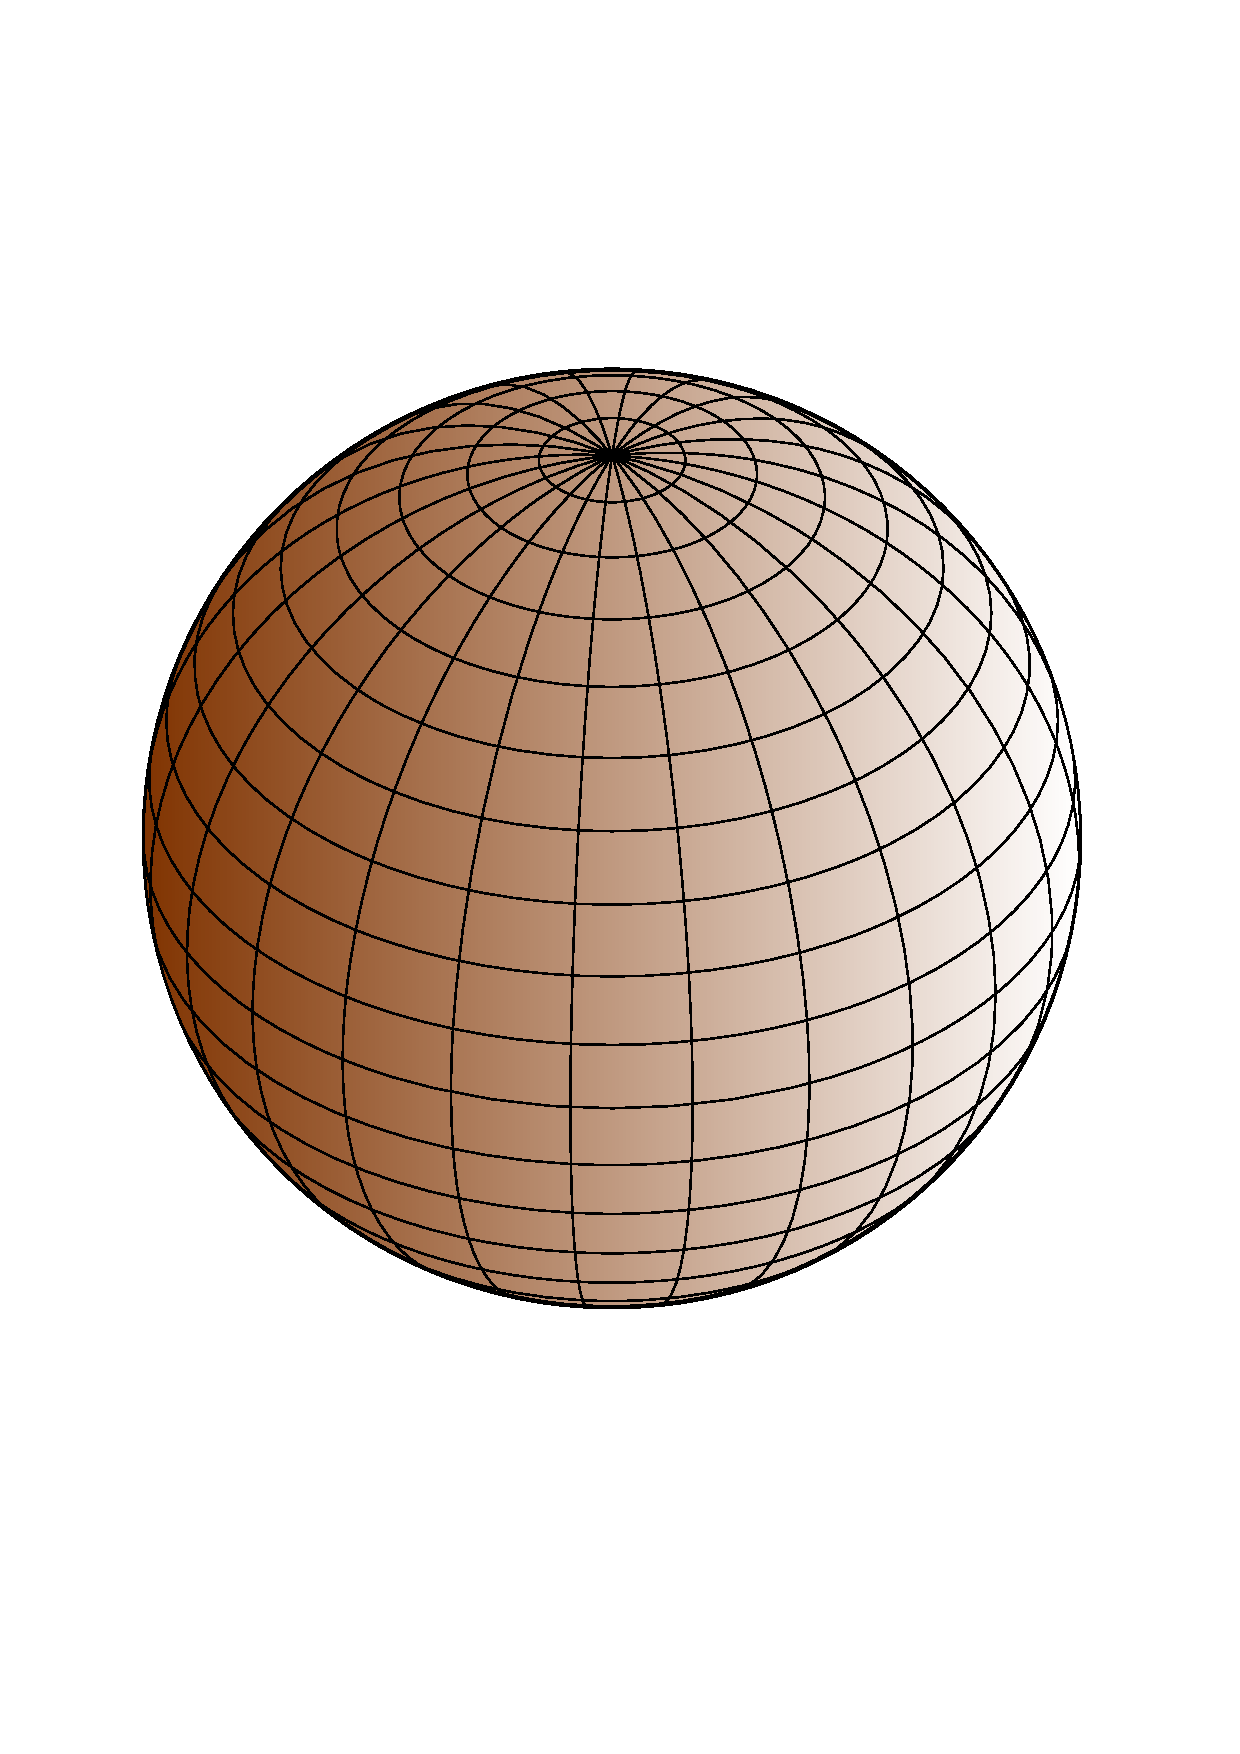
\includegraphics[height=\textwidth]{sphere}
        \caption{Constant scalar curvature}
    \end{subfigure}%
    ~ 
    \begin{subfigure}[t]{0.4\textwidth}
        \centering
        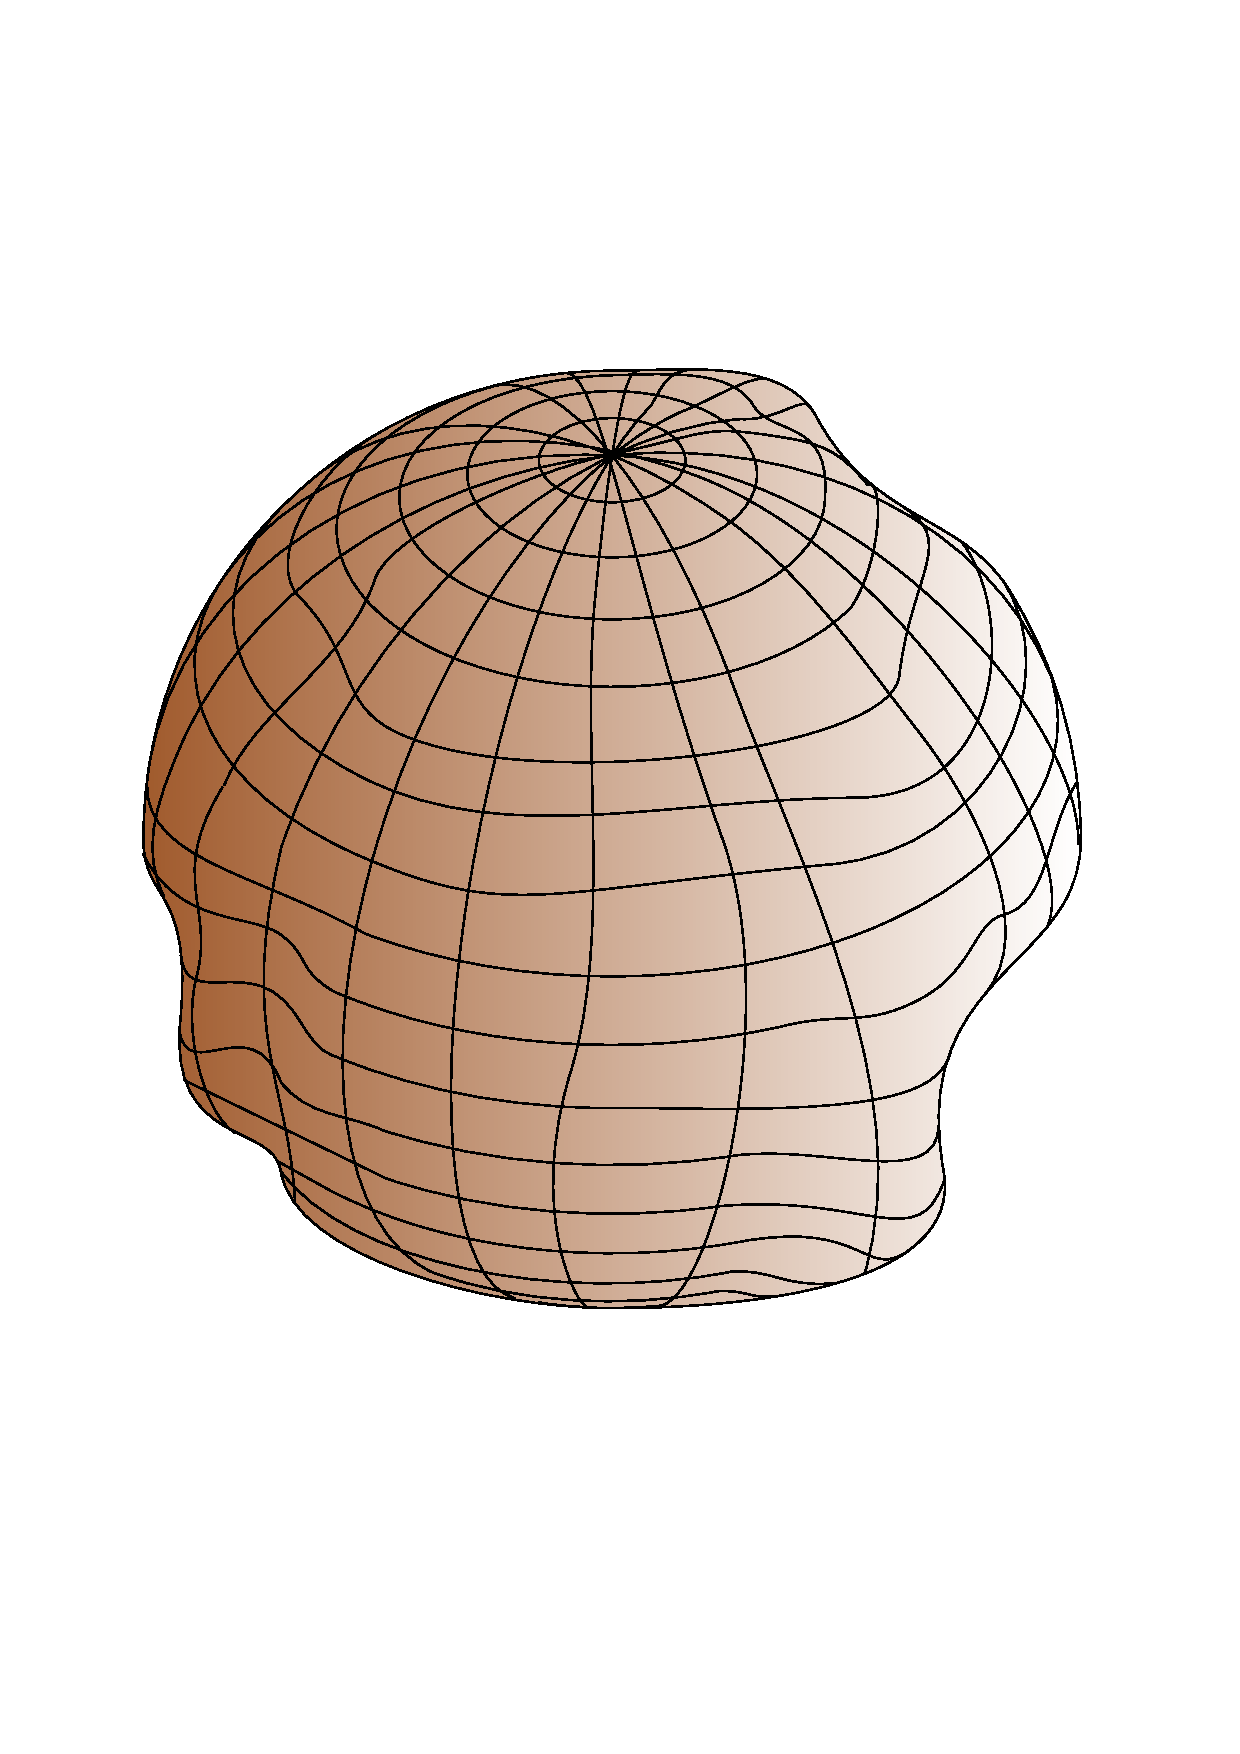
\includegraphics[height=\textwidth]{notsphere}
        \caption{non-constant scalar curvature}
    \end{subfigure}
    \caption{two choices of metric on \(S^2\)}
\end{figure*}


In \cite{calabi54,calabi57}, Calabi proved certain results for compact K\"ahler manifolds which lead to a famous conjecture. Fix a compact K\"ahler manifold \((X,\omega)\). Recall that the Ricci curvature form \(\Ric(\omega)\) is a real \((1,1)\)-form and defines a characteristic class \(c_1(X) = \frac{1}{2 \pi} [ \Ric(\omega)] \) of the manifold, known as the first Chern class. Calibi asked whether, given a real \((1,1)\)-form \( \eta \) representing the first Chern class of \(X\), can we find a unique K\"ahler metric \(\omega'\) in the same cohomology class as \(\omega\) such that \(\Ric(\omega') = 2 \pi \eta\)?

A related conjecture asked whether all compact K\"ahler manifolds \((X,\omega)\) admit a K\"ahler-Einstein metric, or more specifically whether they admit a K\"ahler form \(\omega'\) in the same cohomology class as \(\omega\) with \(\Ric \omega' = \lambda \omega'\), for some real constant \(\lambda\). This equation is known as the Einstein condition\footnote{as it is analogous to Einstein's field equations in a vacuum.}, and the K\"ahler metric corresponding to \(\omega'\) is called a K\"ahler-Einstein metric. (metric of constant scalar curvature) It follows that for \(X\) to admit such a metric, \(\Ric \omega'\) must be a definite \((1,1)\)-form. This separates the problem into three cases: positive definite, zero, and negative definite. In the first two cases K\"ahler-Einstein metrics on \(X\) are precisely the metrics of constant scalar curvature, and so one may see this as a direct generalization of the uniformization theorem for Riemann surfaces.

Aubin \cite{Aubin1976} and Yau \cite{Yau1977} settled the negative definite case first. Calibi's conjecture was also proven by Yau in \cite{Yau1977}, later contributing to him being awarded the fields medal. This left the positive definite case, which correspond to smooth Fano varieties under the Kodeira embedding theorem. It was already known however, due to Matsushima \cite{matsushima1957structure}, that not all Fano manifolds were K\"ahler-Einstein. It then became an objective to find suitable criterion for the existence of a K\"ahler-Einstein metric on a Fano manifold.

Matsushima had shown that necessary condition for a K\"ahler-Einstein metric was reductivity of the automorphism group of the manifold. In \cite{futaki1983obstruction} Futaki introduced a new invariant whose vanishing was also a necessary condition. In \cite{tian1987kahler} Tian introduced a sufficient condition in terms of another invariant, known now as \textit{Tian's alpha invariant}.
Tian's alpha invariant is a generalization of the complex singularity exponent of a polynomial \(f \in \CC[z_1,\dots,z_n]\), which is defined as follows:
\[
c_O(f) := \sup \{ \epsilon | \ |f|^{-2 \epsilon} \text{ integrable  in a neighborhood of } O \in \CC^n \} .
\]
The Yau-Tian-Donaldson conjecture suggested the notion of \textit{ \(K\)-stability} as a necessary and sufficient K\"ahler-Einstein criterion\footnote{In full, the YTD talks of csck metrics, which are equivalent to KE in the Fano case}. This was proven in the trilogy of papers \cite{chen2015kahler1,chen2015kahler2,chen2015kahler3}.

A generalization of the notion of a K\"ahler-Einstein metric is a K\"ahler-Ricci soliton. To understand how, recall that K\"ahler Einstein metrics may be seen as generalized fixed point solutions under the K\"ahler-Ricci flow:
\[
\frac{d}{dt} \omega_t = -2 \Ric(\omega_t)
\]
In that under this flow they will remain unchanged up to some scaling factor. A K\"ahler-Ricci soliton is a generalized fixed point of the flow in the sense that it will remain unchanged up to some diffeomorphism (biholomorphism? check). (references for different things here)

A further generalization are twisted K\"ahler-Einstein metrics and twisted K\"ahler-Ricci solitons. These arise in continuity method arguments, see \cite{datar2016kahler} for example, and depend on a parameter \(t \in [0,1]\). Here we start with a Calibi-Yau type solution \(\omega_0\) at \(t=0\), and consider the existence of solutions \(\omega_t\) along a line segment to the target K\"ahler-Einstein or K\"ahler-Ricci soliton equation at \(t= 1\) respectively. The supremum of the set of \(t\) for which a solution exists turns out to be independent of \(\omega_0\), and of a lot of interest as an invariant of \(X\). It is often called the beta invariant, or the greatest lower bound on Ricci curvature. We will denote this invariant by \(R(X)\).

Although \(K\)-stability is a criterion for the existence of K\"ahler-Einstein metrics and various generalizations, it is not an effective one. In general the \(K\)-stability of a Fano manifold is difficult to calculate. The alpha invariant approach also has limitations in practice. Fortunately equivariant versions of \(K\)-stability and Tian's alpha invariant exist, which, as we will see, provide an effective approach in classes of manifolds and orbifolds with lots of symmetry.

One class in particular we will explore is the class of Fano manifolds and orbifolds which are also \(T\)-varieties. A \(T\)-variety is a normal variety which admits the effective action of an algebraic torus \(T = (\CC^*)^r\). These are a generalization of toric varieties, where \(\dim T = \dim X\). In general we call the difference \(\dim X - \dim T\) the complexity of the torus action.

In the toric case it is well-established that studying \(X\) is equivalent to studying some associated combinatorial data: a fan of cones in a vector space built from the cocharacter lattice of \(T\). Thanks to the work of many authors (Altmann, Hausen, Ilten, Petersen, S\"u\ss, Vollmert to name a few) this combinatorial description extends to higher complexity.

Equivariant methods have been used to provide some effective criteria for canonical metrics on low complexity \(T\)-varieties. If \(X\) is a Fano toric variety then the problem is completely solved. In \cite{wang2004} it was shown that \(X\) is K\"ahler-Einstein if and only if the Futaki character vanishes. They showed also that the Futaki character coincides with the barycenter of the lattice Polytope corresponding to \(X\). Wang et al did not use \(K\)-stability for this result, but the result was later reproven as an application of the main theorem of \cite{datar2016kahler}.

In \cite{ilten2015}, Suess and Ilten considered the \(K\)-stability of \(T\)-varieties of complexity one. We recall this in detail in Section~\ref{prelim:twisted}. Complexity one Fano \(T\)-varieties have a combinatorial description. They obtained a combinatorial criterion for \(K\)-stability, generalizing the results of \cite{wang2004}. S\"u\ss had also used the equivariant version of Tian's alpha invariant to find new K\"ahler-Einstein metrics on complexity one \(T\)-varieties admitting additional symmetries in \cite{suss2013kahler}.

In complexity two and above, even equivariant \(K\)-stability remains an ineffective criterion. In the next section we will give a summary of the new results presented in this thesis, one of which are some new examples of K\"ahler-Einstein \(T\)-manifolds of complexity two. As far as the author is aware, these are first complexity examples to be obtained through equivariant methods.

\section{Content of the Thesis} \label{content}
Here I list the new results presented in this thesis. Some of the content of this thesis has been published and/or submitted to journals, which I will reference. I also make clear, in the case of my coauthored work, the scope of my contribution to the original paper. Chapters 4 and 5 summarize results obtained in my first and second years of my PhD respectively, and are included for completeness and context.
\subsection*{Chapter 3 - New K\"ahler-Ricci solitons on Fano threefolds} \label{content:riccisolitons}
In Chapter~\ref{chap:sol} we consider Fano threefolds admitting an effective \(2\)-torus action within the classification of \cite{mori1981classification}. In \cite{suss2013fano} a not necessarily complete list of such threefolds together with their combinatorial description was given. We extend the results of \cite{ilten2015}, providing new examples of threefolds admitting a non-trivial K\"ahler-Ricci soliton. Recall that a K\"ahler-Ricci soliton on a Fano manifold \((X,\omega)\) is a pair \((\omega',v)\) satisfying:
\[
\Ric(\omega') - L_v \omega' = \omega'
\]
We apply some real interval arithmentic approximations to the complexity one formula for the Futaki invariant of Ilten and Suess (see Section~\ref{subsec:IS}) to check the existence criterion \cite{datar2016kahler} (see Section~\ref{prelim:twisted}). We include the relevant Sagemath code in Appendix~\ref{App:code}.
\subsection*{Chapter 4 - The greatest lower bound on Ricci curvature in complexity one} \label{content:R(X)}
In Chapter~\ref{chap:R(X)} we present an explicit effective formula obtained for the greatest lower bound on Ricci curvature \(R(X)\) for a complexity one \(T\)-variety \(X\). We follow the authors work \cite{cable2019greatest}. These results generalize a result of Li \cite{li2009greatest}, but the proof uses results of \(G\)-equivariant \(K\)-stability from \cite{datar2016kahler}. The invariant \(R(X)\) is often denoted \(\beta(X)\) and is referred to as Tian's beta invariant. By \cite{} is now known to coincide with another important invariant, \(\delta(X)\).
\subsection*{Chapter 5 - New K\"ahler-Einstein metrics on symmetric general arrangement varieties} \label{content:generalarrangement}
In Chapter~\ref{chap:gav}, we discuss recent results obtaining new K\"ahler-Einstein metrics on some symmetric complexity two general arrangement varieties. General arrangement varieties are \(T\)-varieties where the torus quotient is a projective space, and the critical values of the quotient map form a general arrangement of hyperplanes in that projective space. Smooth general arrangement varieties of complexity and Picard rank \(2\) were classified according to their Cox ring in \cite{hausen2018torus}. Following the methods of \cite{Su13}, we find three new examples of K\"ahler-Einstein metrics. As far as we are aware, these are the first examples of K\"ahler-Einstein metrics found on \(T\)-varieties of complexity greater than one by way of equivariant methods.